
\section{Methodology}

\subsection{Participants}




\subsection{Procedure}

The procedure unfolded in a systematic fashion to facilitate a comprehensive exploration of participants' perceptions and interactions with the envisioned musical plants. Upon welcoming each participant, we presented them with the intriguing premise: "We're in the very near future. You are looking at plants that make music when you physically interact with them (it is not actually the case, but imagine it). Explore their capabilities." This imaginative prompt aimed to elicit uninhibited responses and creative engagement. Subsequently, participants were given the freedom to explore the potential musical capacities of the plants at their own pace. An important aspect of the procedure was our deliberate decision not to provide any guidance or answer questions during the exploration phase, allowing for unfiltered and spontaneous reactions. In instances where participants encountered difficulty initiating exploration, the prompt was reiterated to encourage a more immersive and uninhibited interaction with the conceptualized musical flora. This methodological approach was designed to capture the unmediated and diverse responses of participants as they navigated the uncharted territory of human-plant interaction. Also, we avoided any kind of communication or talking between 2 participants to reduce the potential bias.


\subsection{Materials/Tools}

To proceed and conduct this user study, we choose 3 different plants from 3 different species.

\newpage

\subsubsection{Dracaena}
They project was initially conducted using this specific plant. It has long leaves and fragile perceived trunk but also flexible.

\begin{figure}[h!]
    \centering
    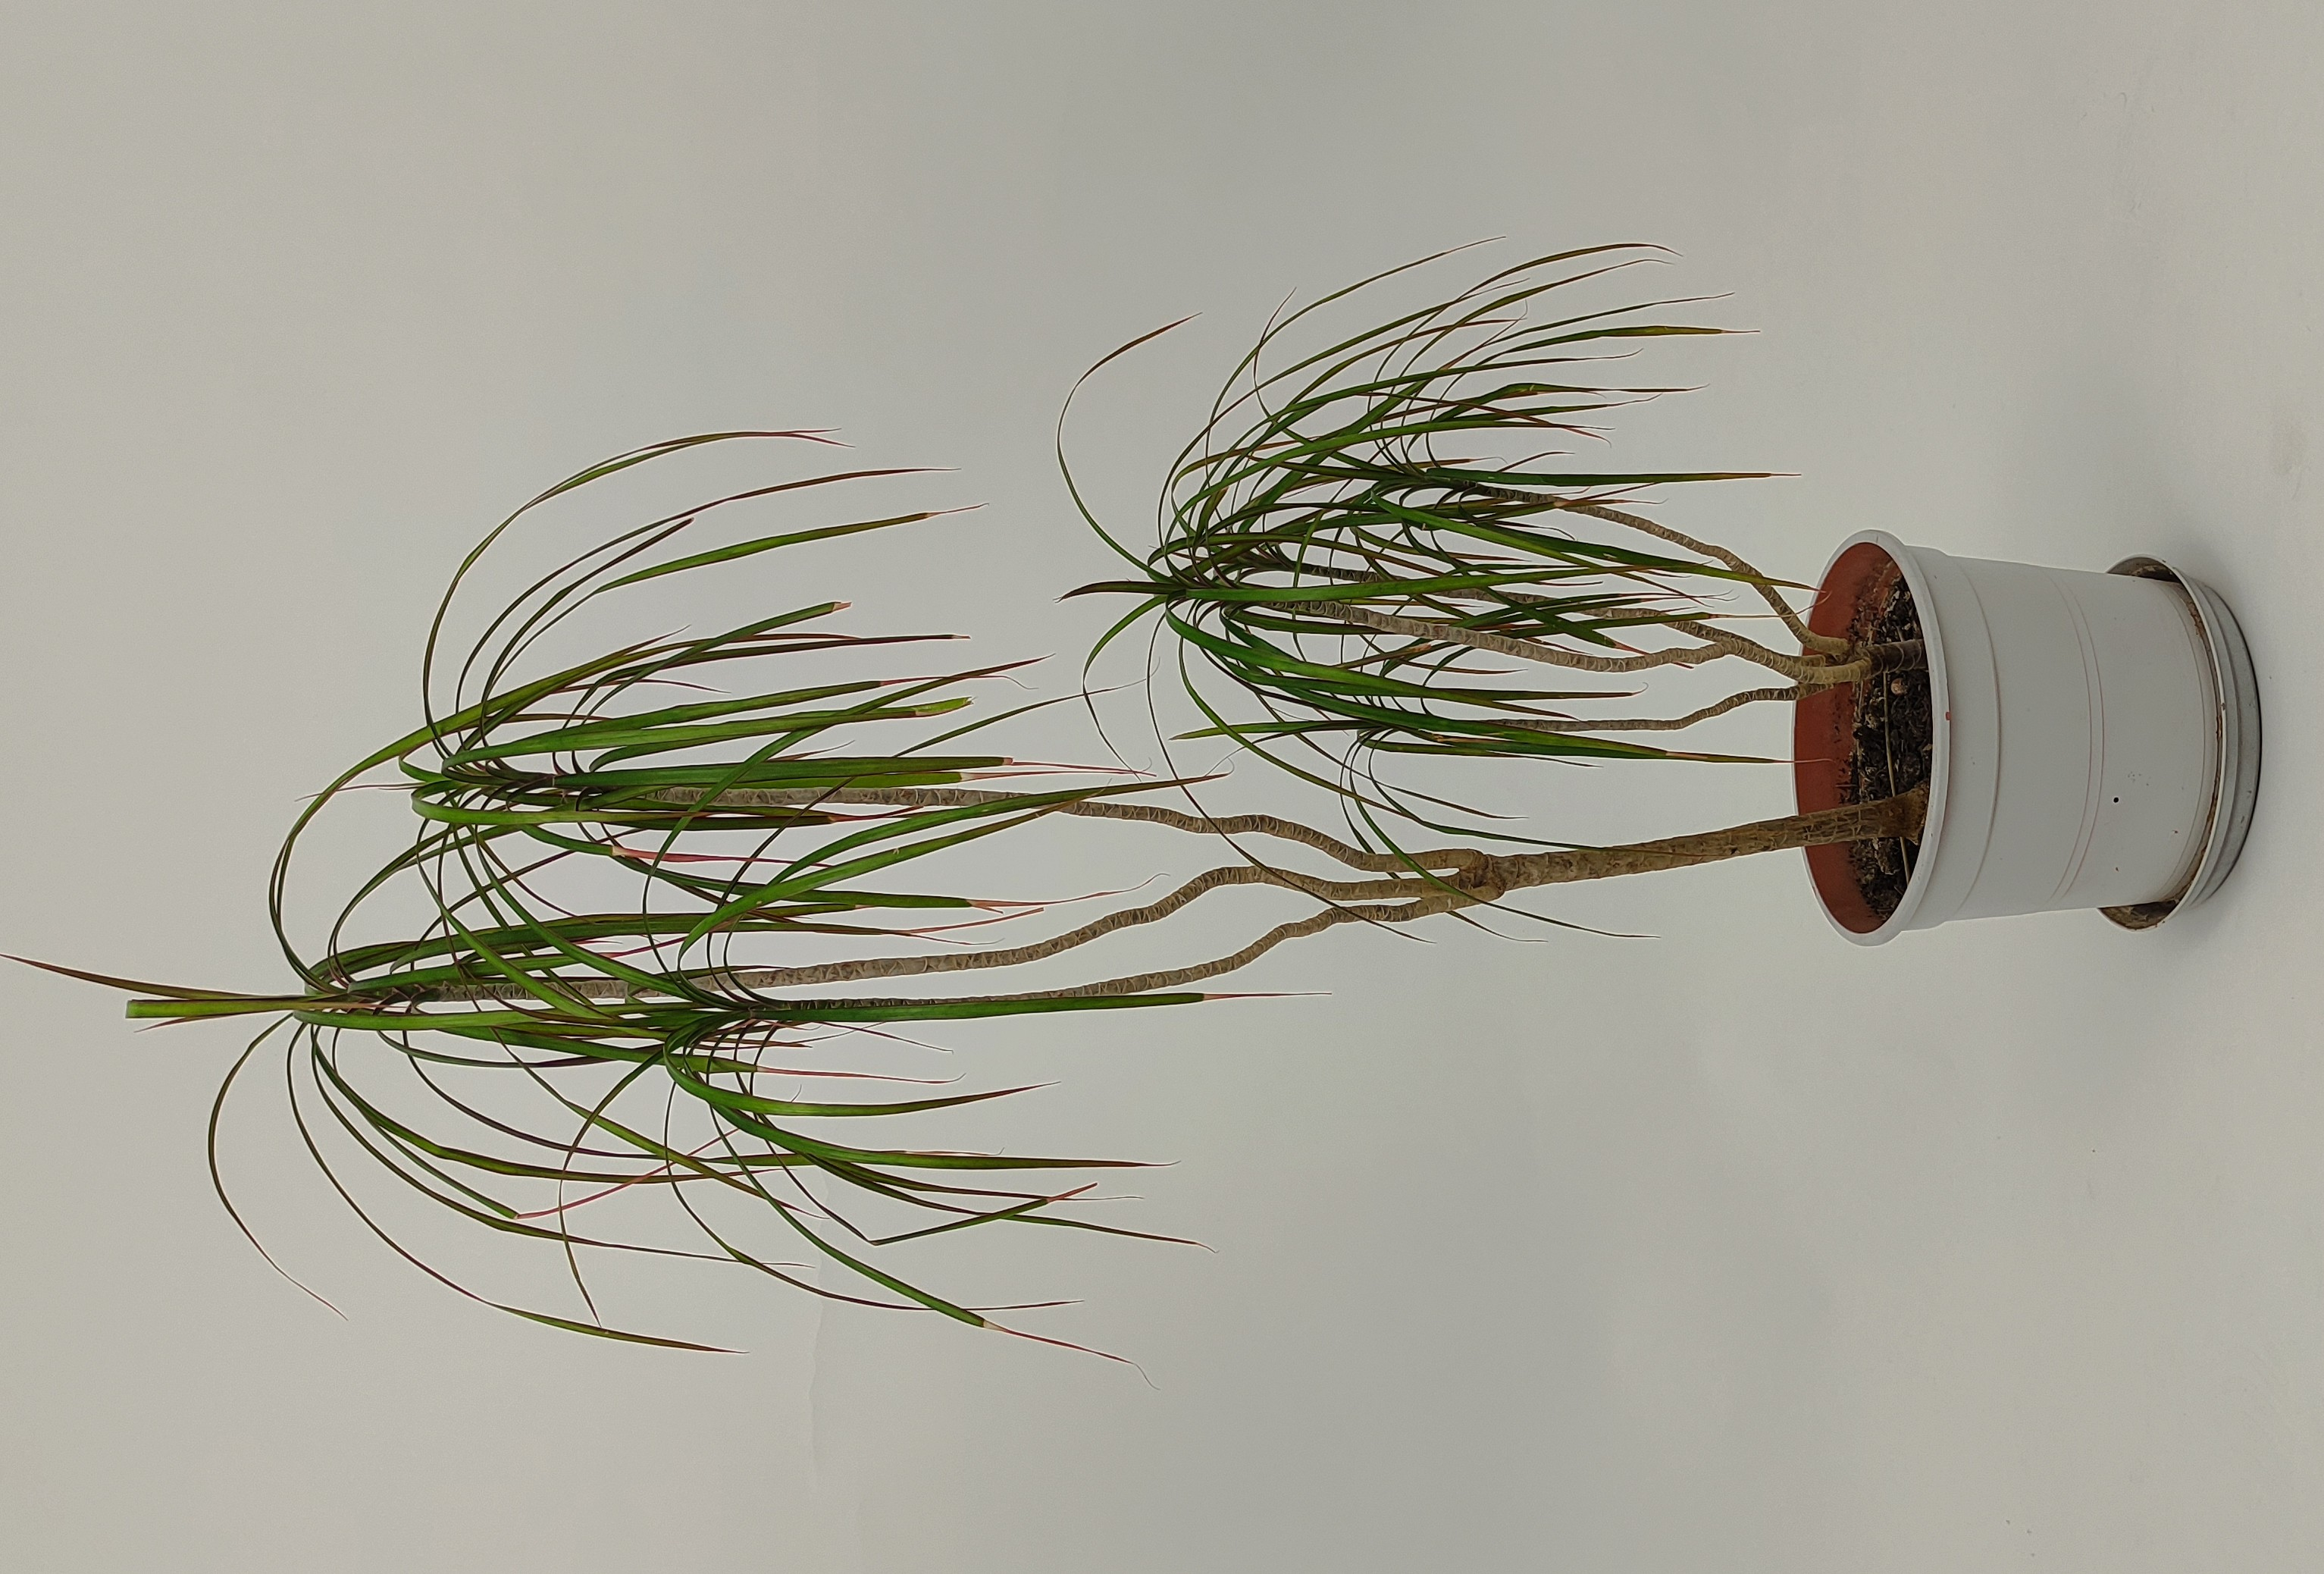
\includegraphics[width=0.42\textwidth, angle=-90]{Images/small_plant.jpg}
    \caption{The N°1 plant is a \textit{Dracaena}.}
    
    \vspace{-0.5cm}
    \label{fig:small_plant}
    \vspace{0.2cm}
\end{figure}




\subsubsection{Pachira glabra}

We chose to use this plant for its large leaves and its wide trunk. This \textit{Pachira} is a bit taller than the \textit{Dracaena} (figure \ref{fig:small_plant}).
\begin{figure}[h!]
    \centering
    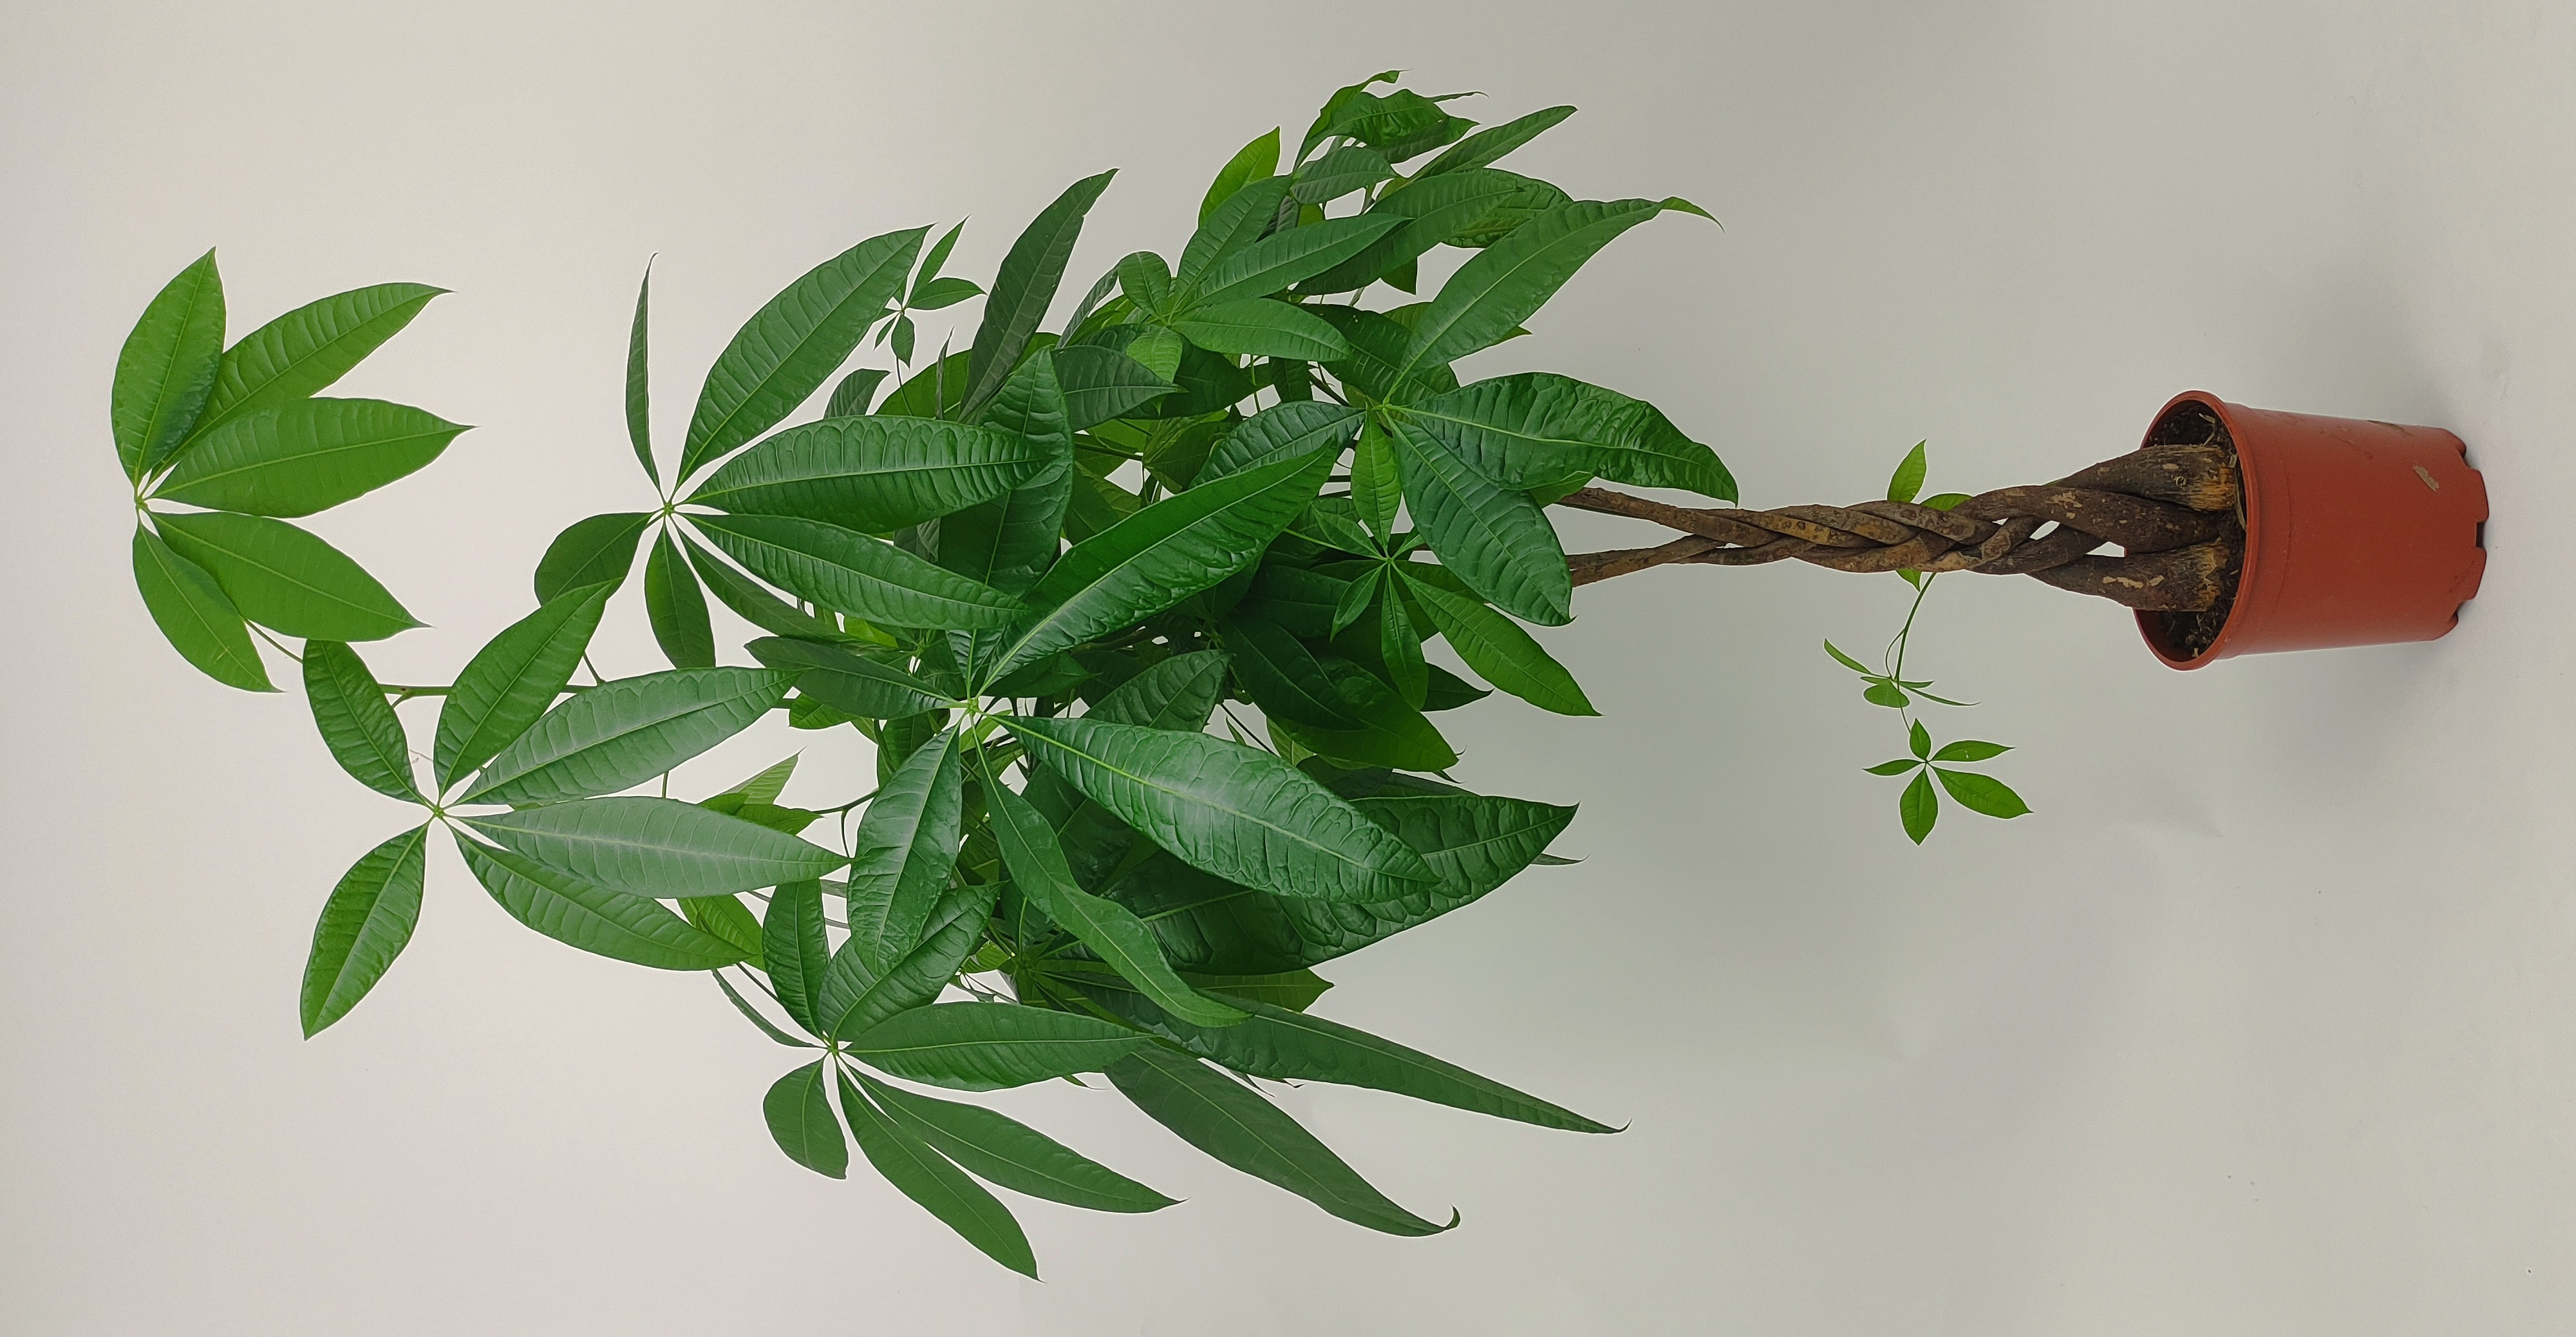
\includegraphics[width=0.42\textwidth, angle=-90]{Images/tall_plant_cropped.jpg}
    \caption{The N°2 plant is a \textit{Pachira glabra}.}
    
    \vspace{-0.5cm}
    \label{fig:tall_plant}
    \vspace{0.2cm}
\end{figure}


\newpage

\subsubsection{Dypsis lutescens}

The \textit{Dypsis lutescens} is very different from the two other plants. Indeed, it is composed of many trunks and stems. On top of that, the leaves are numerous and tight.

\begin{figure}[h!]
    \centering
    \includegraphics[width=0.42\textwidth, angle=-90]{Images/fougere_plant.jpg}
    \caption{The N°3 plant is a \textit{Dypsis lutescens}.}
    
    \vspace{-0.5cm}
    \label{fig:fougere_plant}
    \vspace{0.2cm}
\end{figure}



\subsubsection{The experimental space}

The experimental space served as an open canvas for the exploration of human-plant interaction within the Internet of Plant project. While the configuration was not explicitly tailored to the plants, it provided a versatile environment that accommodated the envisioned musical flora. The space featured three distinct levels of height, each corresponding to one of the three plants introduced to participants. 

\begin{figure}[h]
    \centering
    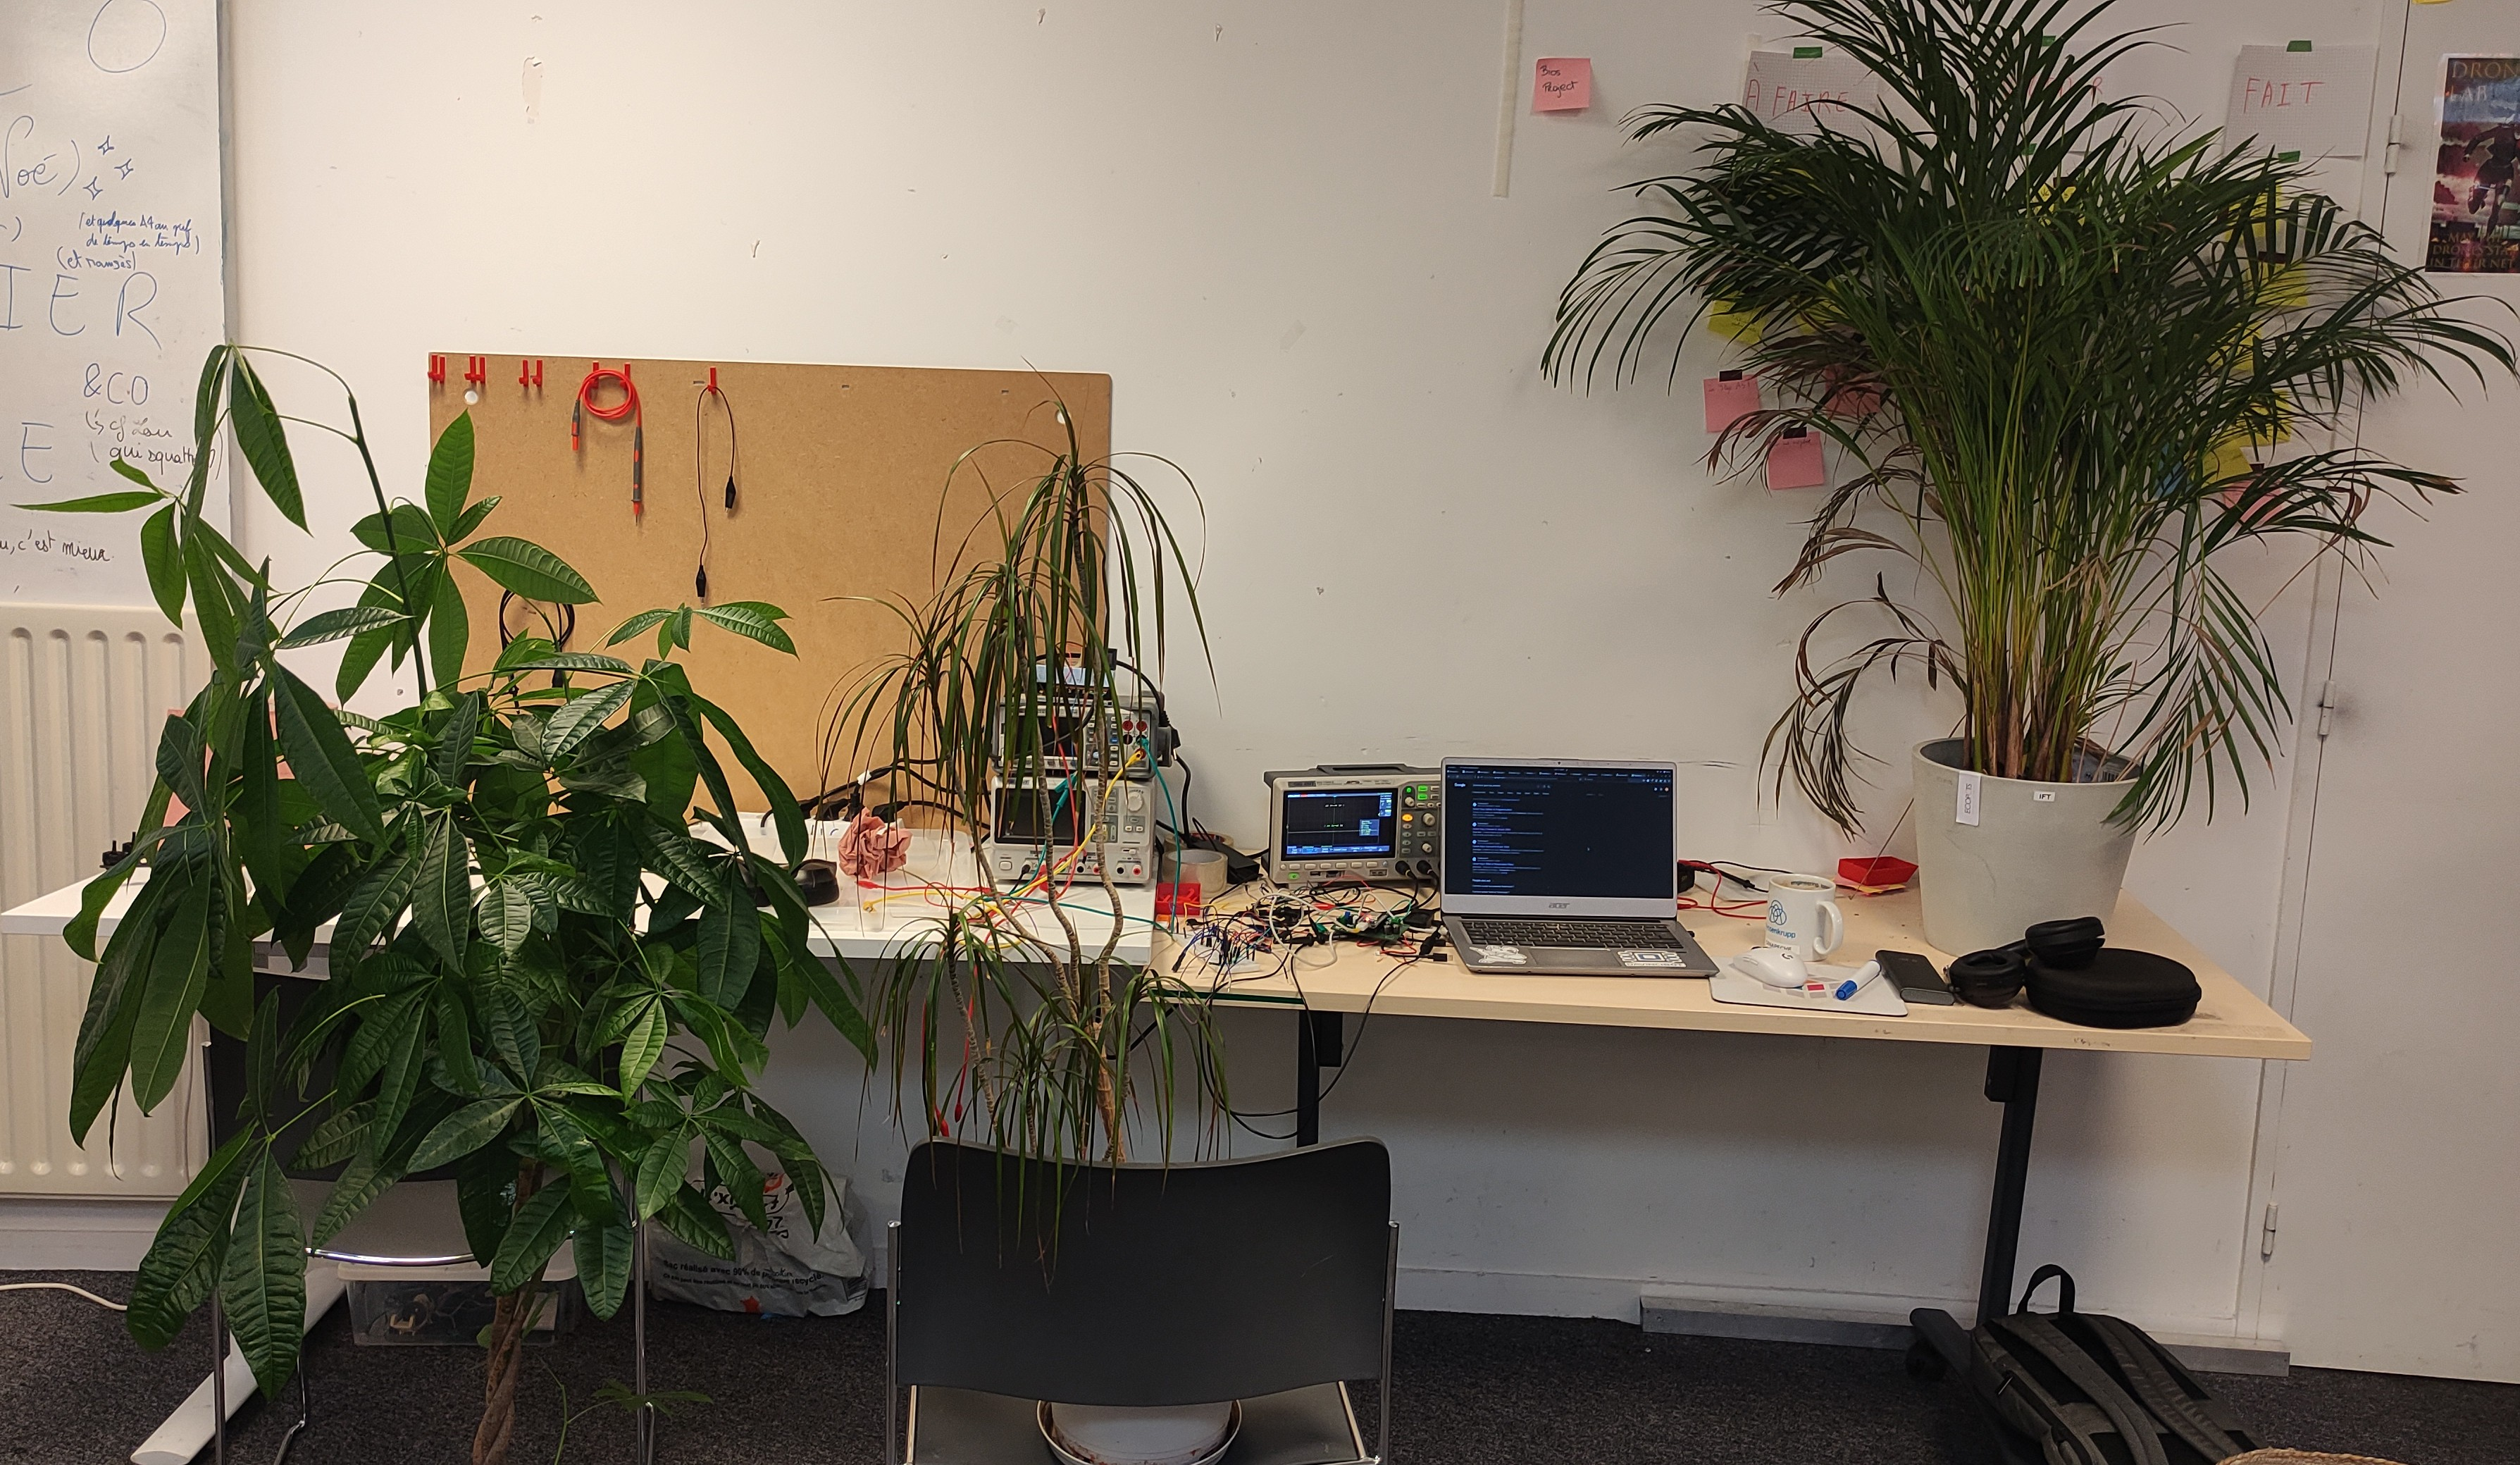
\includegraphics[width=0.42\textwidth]{Images/setup_user_study.jpg}
    \caption{User study space setup. The setup is built from our lab space.}
    
    \vspace{-0.5cm}
    \label{fig:setup_user_study}
    \vspace{0.2cm}
\end{figure}

\newpage

